\documentclass[tikz]{standalone}

\usetikzlibrary{calc,quotes,angles,patterns,babel}

\usepackage{amsmath,amssymb}

\newcommand{\richtungsfeld}[8]{ %#1: xmin #2: xmax #3: ymin #4: ymax #5: stepsize #6: differentialequation for x #7: differentialequation for y #8: scaling factor for arrows
	\foreach \x in {#1,{#1+#5},...,#2}{
		\foreach \y in {#3,{#3+#5},...,#4}{
			\draw[->] ({\x-(#8)*(#6)/2},{\y-(#8)*(#7)}/2)--++({(#8)*(#6)},{(#8)*(#7)});
		}
	}
}

\begin{document}
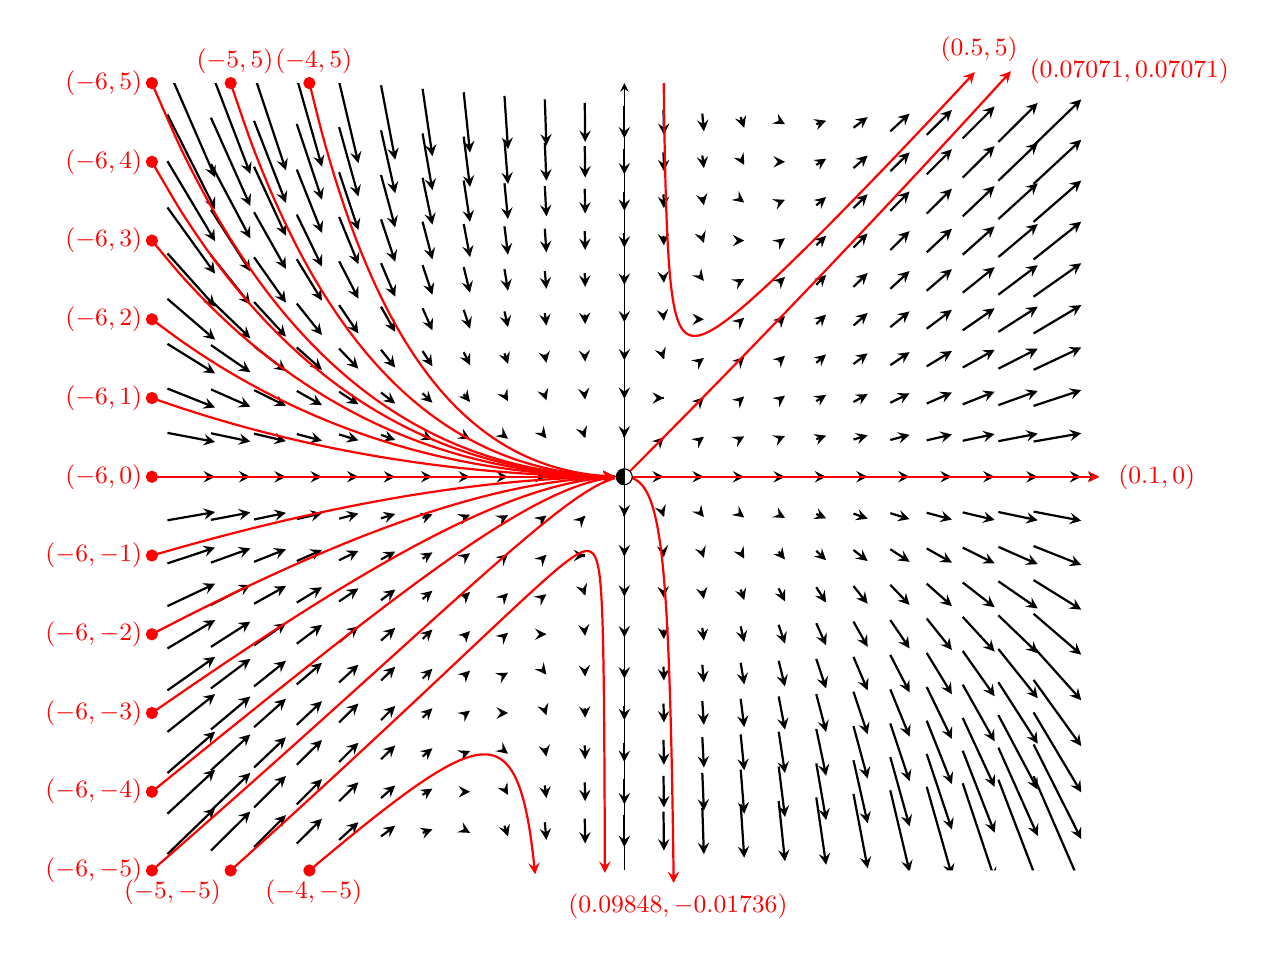
\begin{tikzpicture}[>=stealth]
	\draw[->] (-6,0)--(6,0);
	\draw[->] (0,-5)--(0,5);
	\def\s{0.02};
	\begin{scope}
		\clip (-0.2,-0.2)--(-0.2,0.2)--(0.2,0.2)--(0.2,-0.2)--(-0.2,-0.2)(-6,-5)--(6,-5)--(6,5)--(-6,5)--(-6,-5);
		\foreach \x in {-5.5,-5,...,5.5}{
			\foreach \y in {-4.5,-4,...,4.5}{
				\draw[->,thick] ({\x-(\s)*((\x)^2)/2},{\y-(\s)*(\y*(2*\x-\y))/2})--({\x+(\s)*((\x)^2)/2},{\y+(\s)*(\y*(2*\x-\y))/2});
			};
		};
	\end{scope}
	\xdef\mylist{-4/-5}
	\foreach \x in {-5,-6} \xdef\mylist{\mylist,\x/-5};
	\foreach \x in {-4,...,5} \xdef\mylist{\mylist,-6/\x};
	\foreach \x in {-5,-4} \xdef\mylist{\mylist,\x/5};
	\foreach \x/\y [evaluate=\x,evaluate=\y] in {0.1*cos(-10)/0.1*sin(-10),0.5/5,0.1/0,0.1*cos(-45)/0.1*sin(45)} \xdef\mylist{\mylist,\x/\y};
	\foreach \x/\y/\z in \mylist {
		\ifdim \x pt = -6pt
			\draw[fill=red,red] (\x,\y)circle(2pt)node[left]{\begin{small} $(\x,\y)$\end{small}};
		\fi
		\ifdim \y pt = -5pt
			\ifdim \x pt = -5pt 
				\draw[fill=red,red] (\x,\y)circle(2pt)node[below left]{\begin{small} $(\x,\y)$\end{small}};
			\fi
			\ifdim \x pt = -4pt 
				\draw[fill=red,red] (\x,\y)circle(2pt)node[below]{\begin{small} $(\x,\y)$\end{small}};
			\fi
		\fi
		\ifdim \y pt = 5pt
			\ifdim \x pt > -6pt
				\ifdim \x pt < 0pt
					\draw[fill=red,red] (\x,\y)circle(2pt)node[above]{\begin{small} $(\x,\y)$\end{small}};
				\fi
			\fi
		\fi
		\pgfmathsetmacro{\stepx}{0.01}
		\pgfmathsetmacro{\myx}{\x}
		\pgfmathsetmacro{\myy}{\y}
		\xdef\listdat{(\x,\y)}
		\ifdim \x pt < -1pt
			\def\helpme{800}
		\fi
		\ifdim \x pt > -1pt
			\def\helpme{2000}
		\fi
		\foreach \k in {1,...,\helpme}{
			\pgfmathsetmacro{\myx}{\myx+\stepx*(\myx*\myx)}
			\pgfmathsetmacro{\myy}{\myy+\stepx*(\myy*(2*\myx-\myy))}
			\xdef\myx{\myx}
			\xdef\myy{\myy}
			\xdef\listdat{\listdat (\myx,\myy)}
			\ifdim \myx pt < -6pt
				\breakforeach
			\fi
			\ifdim \myx pt > 6pt
				\breakforeach
			\fi
			\ifdim \myy pt < -5pt
				\breakforeach
			\fi
			\ifdim \myy pt > 5pt
				\breakforeach
			\fi
		}
		\ifdim \x pt < -3pt
			\draw[red,thick,->] plot[smooth] coordinates {\listdat};
		\fi
		\ifdim \x pt > -3pt
			\ifdim \y pt = 5pt
				\draw[red,thick,->] plot[smooth] coordinates {\listdat} node[above]{\begin{small} $(\x,\y)$\end{small}};
			\fi
			\ifdim \y pt < 0pt
				\draw[red,thick,->] plot[smooth] coordinates {\listdat} node[below]{\begin{small} $(\x,\y)$\end{small}};
			\fi
			\ifdim \y pt < 5pt
				\ifdim \y pt > -0.01pt
					\draw[red,thick,->] plot[smooth] coordinates {\listdat} node[right]{\begin{small} $(\x,\y)$\end{small}};
				\fi
			\fi
		\fi
	}
	\draw[black,fill=white] (0,0)circle(0.1cm);
	\draw[fill=black] (0,0)--(0,0.1)arc(90:270:0.1cm)--(0,0);
\end{tikzpicture}
\end{document}
